% Capítulo 9 — Descomposición en valores singulares: la base privilegiada y el terreno
\chapter{Descomposición en valores singulares: la base privilegiada y el terreno}\label{cap:09}

\section{La idea}

% --- 09-svd-nivel1 (redactado 2026-10-18) ---
\subsection{Una base para la entrada, otra para la salida}\label{sec:svd-idea}

\paragraph{La pregunta que cambia.} En el capítulo de álgebra buscamos las direcciones que
una transformación deja caer sobre sí mismas, los autovectores, y con ellas escribimos la
matriz como diagonal: \(A=PDP^{-1}\) (sección~\ref{sec:cambio-base}). La idea es buena y
tiene tres defectos que ya vimos. Una rotación no deja ninguna recta real fija; un corte deja
una sola; una matriz rectangular, que lleva el plano a \(\R^3\) o \(\R^3\) al plano, ni
siquiera puede preguntarse qué vectores caen sobre sí mismos, porque la entrada y la salida
son espacios distintos. La descomposición en valores singulares (SVD, por sus siglas en
inglés) cambia la pregunta: en lugar de una sola base que sirva a la vez para la entrada y
para la salida, buscamos \emph{dos} bases ortonormales, una en cada espacio, elegidas de
manera que la transformación lleve la primera sobre la segunda estirando cada eje por
separado. En esas dos grillas cualquier matriz, cuadrada o rectangular, con autovalores
reales o sin ellos, es una matriz diagonal con entradas no negativas:
\[
  A=U\,\Sigma\,V^T,\qquad
  V:\ \text{base de la entrada},\quad
  \Sigma:\ \text{estirar cada eje},\quad
  U:\ \text{base de la salida}.
\]
Lo que se gana es generalidad; lo que se pierde es la posibilidad de componer la
transformación consigo misma en esa base, porque la grilla de llegada no es la de partida.

\paragraph{Hecho geométrico: lo redondo se vuelve elipse.} La forma más directa de ver las
dos bases es mirar qué hace la transformación con todas las direcciones a la vez.

\begin{itemize}
  \item En \(\R^2\), la circunferencia unidad va a parar a una elipse (o, si la matriz
  aplasta, a un segmento). Los largos de los semiejes de esa elipse son los \emph{valores
  singulares} \(\sigma_1\ge\sigma_2\ge0\); las direcciones de los semiejes son las columnas
  de \(U\); las dos direcciones perpendiculares de la circunferencia que terminan sobre esos
  semiejes son las columnas de \(V\). Toda elipse tiene un par de ejes perpendiculares, y
  por eso la SVD existe siempre.
  \item En \(\R^3\), la esfera unidad va a parar a un elipsoide: tres semiejes
  perpendiculares, tres valores singulares, tres direcciones de llegada en \(U\) y tres de
  partida en \(V\). Si un \(\sigma\) es cero, el elipsoide se aplastó a una elipse plana, y
  la dirección de partida correspondiente es el núcleo.
  \item En una matriz de \(m\times n\), la esfera de \(\R^n\) va a parar a un elipsoide,
  posiblemente aplastado, dentro de \(\R^m\). La cantidad de semiejes no nulos es el rango.
  Las direcciones de \(\R^n\) que se aplastan forman el núcleo y las direcciones de
  \(\R^m\) que la elipse no alcanza forman el espacio inaccesible: los cuatro subespacios
  de la sección~\ref{sec:pseudoinversa} salen de la misma figura.
\end{itemize}

Leída de derecha a izquierda, la descomposición dice que toda transformación lineal es un
giro (o una reflexión) de la entrada, seguido de estiramientos sobre los ejes, seguido de un
giro (o una reflexión) en la salida. Los giros no cambian largos; todo lo que la
transformación hace con las distancias está concentrado en los números de \(\Sigma\).

\paragraph{Por qué el profesor la llama ``base privilegiada''.} Para el profesor, el punto
de partida de la SVD es encontrar una ``base privilegiada'' de la transformación (resumen
2025, clase 7). La palabra tiene peso, porque el mismo curso insiste en que, en abstracto,
``no existe una base vectorial privilegiada de \(\R^n\), y lo único que define a la base que
llamamos canónica es que sobre ella tenemos definida la noción de distancia a través del
producto interno'' (resumen 2025, clase 6). Y lo repite al hablar de cambio de base: ``En un
espacio vectorial donde la magnitud de un vector no sea algo que esté definido o que
importe, la base canónica no tiene nada especial'' (resumen 2025, clase 8).

Ahí está la clave. La SVD pide bases \emph{ortonormales}: vectores de largo uno y
perpendiculares entre sí. Largo y perpendicularidad no los da la transformación sino el
producto interno de cada espacio. Sin producto interno, una circunferencia no se distingue
de una elipse y no hay semiejes que medir; con producto interno, la elipse imagen tiene ejes
bien definidos y esos ejes eligen las bases. Por eso la base que la SVD privilegia no es
privilegiada por la matriz sola, sino por la matriz junto con las dos reglas de medir, la de
la entrada y la de la salida (sección~\ref{sec:puntos-formas-grillas}). Si cambiamos la
regla, cambian los valores singulares. Un ejemplo que vamos a usar con el terreno: la
transformación que lleva un desplazamiento de \((\Delta\text{columnas},\Delta\text{filas})\)
de una grilla geográfica a metros sobre el suelo es, en el recorte de la Precordillera,
\(\operatorname{diag}(26{,}19;\ 30{,}80)\), porque a \(32^\circ\) de latitud un segundo de longitud mide
aproximadamente \(\cos\varphi\approx0{,}85\) veces lo que mide un segundo de latitud. Para quien cuenta
celdas los dos ejes son iguales; para quien mide en metros, la circunferencia de radio una
celda es una elipse de semiejes \(30{,}80\) y \(26{,}19\) m.

\paragraph{Una herramienta, varios problemas de la materia.} La SVD reúne en una sola
cuenta preguntas que en el programa aparecen separadas. Cada una se contesta mirando una
parte distinta de \(U\Sigma V^T\):

{\small
\begin{center}
\begin{tabularx}{.94\textwidth}{>{\raggedright\arraybackslash}p{.42\textwidth} Y}
\toprule
Pregunta de campo & Qué parte de la SVD la contesta\\
\midrule
¿Cuántas de mis ecuaciones son de verdad independientes? ¿Un error chico en los datos se
vuelve un error grande en el resultado? &
cuántos \(\sigma_i\) son no nulos (el rango) y el cociente \(\sigma_1/\sigma_n\) (el
número de condición)\\
Tengo más observaciones que incógnitas y el sistema no cierra (una poligonal, un ajuste) &
la pseudoinversa \(A^{+}=V\Sigma^{+}U^T\): invertir los \(\sigma_i\) no nulos y descartar
lo que cae en el espacio inaccesible\\
Tengo los mismos puntos medidos en dos sistemas locales y busco el giro que mejor los
superpone (Procrustes) &
las dos bases \(U\) y \(V\) de una matriz chica armada con los datos; los \(\sigma_i\) no
intervienen en el giro\\
Ajusto una recta o un plano a una nube con error en todas las coordenadas (regresión total) &
el vector singular del \emph{menor} \(\sigma\): la dirección en que la nube es más delgada\\
¿Qué parte de un relieve es forma grande y qué parte es detalle? ¿Con qué precisión dibujo
sus curvas de nivel? &
los primeros términos \(\sigma_iu_iv_i^T\) de la matriz de alturas y la suma de los
\(\sigma_i^2\) que se descartan (sección~\ref{sec:svd-dem})\\
\bottomrule
\end{tabularx}
\end{center}
}

Las cuatro primeras filas se resuelven en las secciones~\ref{sec:pseudoinversa}
y~\ref{sec:cuatro-problemas}. La última es la que cierra el capítulo: un modelo digital de
elevación es una matriz de alturas, y su SVD separa el relieve en capas ordenadas de mayor
a menor importancia, a partir de las cuales trazamos curvas de nivel tan suaves o tan
detalladas como pida la escala del plano.

\linkUnidad{09_cambio_de_base_svd}{Simulación interactiva: Unidad 13 — Cambio de base, SVD e inversas}

\subsection{Sistemas de ecuaciones y aplicaciones}\label{sec:sistemas-ecuaciones}

El programa incluye sistemas de ecuaciones y ecuaciones de segundo orden. En el contexto de
coordenadas pueden aparecer al:
\begin{itemize}
  \item determinar intersecciones, puntos fijos y parámetros de transformación;
  \item ajustar coordenadas a partir de observaciones redundantes;
  \item describir curvas y superficies cuadráticas;
  \item formular ecuaciones diferenciales sobre superficies.
\end{itemize}

Este bloque deberá precisarse con los enunciados y ejemplos que presente la cátedra. Mientras tanto, los cuatro problemas del esqueleto 2025 (regresión, intersección de círculos, Procrustes, regresión total) están desarrollados, como anticipo, en la sección~\ref{sec:cuatro-problemas}.

\section{Construcciones, cuentas y ejemplos}

Reunimos tres piezas: la SVD, las inversas con los cuatro subespacios y la pseudoinversa, y la guía de los cuatro problemas. No se dictaron en 2C2026; las armamos a partir del resumen 2025 del profesor y de su cuaderno \file{LaSVD.wxmx}, y quedan pendientes de validar.

\subsection{Descomposición en valores singulares (SVD)}\label{sec:svd}

{\small\vspace{1mm}\linkUnidad{09_cambio_de_base_svd}{Simulación interactiva: Unidad 13 — Cambio de base, SVD e inversas}\par}
{\small\vspace{1mm}\linkAnimacion{04_svd_circulo_a_elipse}{Animación: SVD, del círculo a la elipse}\par}


\begin{atencion}[Anticipado]
La SVD no se dictó en 2C2026 (clase 7 del esqueleto; anunciada el 30/9 y el 14/10). Esta
sección se armó antes de que la cátedra la diera, a partir del resumen 2025 del profesor,
de su cuaderno \file{LaSVD.wxmx} y de bibliografía (Strang; Calvetti y Somersalo).
Pendiente de validar.
\end{atencion}

\paragraph{Cambiar la pregunta.} Diagonalizar pregunta qué direcciones caen sobre sí
mismas. Una rotación de \(90^\circ\) no deja ninguna, y el polinomio característico lo dice
con raíces complejas (sección~\ref{sec:autovalores}). El profesor planteó en 2025 que
``podría existir una forma de descomponer la transformación que no tuviera estos
problemas'', y la enunció así: ``siempre existe una base ortogonal del espacio de entrada
de una transformación que se conserva ortogonal a la salida''. La pregunta nueva es:
¿qué direcciones \emph{perpendiculares} de la entrada siguen perpendiculares a la salida?
Esa pregunta siempre tiene respuesta real, porque se construye a partir del producto
interno y no de direcciones fijas.

\paragraph{Hecho geométrico: la circunferencia se vuelve elipse.} Una matriz \(A\) de
\(2\times2\) lleva la circunferencia unidad a una elipse. Los semiejes de la elipse miden
\(\sigma_1\ge\sigma_2\ge0\) (valores singulares); sus direcciones \(u_1,u_2\) son una base
ortonormal de la salida; las direcciones de la circunferencia que van a parar a esos
semiejes, \(v_1,v_2\), son una base ortonormal de la entrada:
\[
  A\,v_i=\sigma_i\,u_i,\qquad
  \boxed{\ A=U\,\Sigma\,V^T\ },\qquad
  U=[u_1\ u_2],\ \ \Sigma=\operatorname{diag}(\sigma_1,\sigma_2),\ \ V=[v_1\ v_2].
\]
Leído de derecha a izquierda: \(V^T\) gira (o refleja) hasta poner \(v_1,v_2\) sobre los
ejes, \(\Sigma\) estira los ejes, \(U\) gira el resultado hasta las direcciones
\(u_1,u_2\). Tres movimientos que ya se entienden por separado. Como \(\Sigma\) es diagonal
con entradas no negativas, no hay giro escondido que arruine la cuenta: los giros se los
llevaron \(U\) y \(V\). Además \(\sigma_1\sigma_2=|\det A|\) (el área de la elipse es la de
la circunferencia por el producto de los semiejes), y \(\sigma_k=0\) significa que la
elipse se aplastó: \(v_k\) está en el núcleo y \(u_k\) queda fuera de la imagen.

Escalera. En \(\R\): \(x\mapsto ax\) se escribe \(a=(\pm1)\cdot|a|\cdot1\); el valor
singular es \(|a|\) y el signo quedó en la ``base de salida''. En \(\R^3\): esfera que se
vuelve elipsoide, tres semiejes. Si la matriz es \(3\times2\), como la jacobiana de una
superficie parametrizada, la circunferencia del plano \((u,v)\) va a una elipse que vive en
el plano tangente dentro de \(\R^3\) y el tercer vector \(u_3\) apunta a la normal, la
dirección inaccesible: \(U\) es \(3\times3\), \(V\) es \(2\times2\), \(\Sigma\) es
\(3\times2\). Es el ``cambio de base rectangular'' que el profesor anunció el 30/9.

\paragraph{Ejemplo a mano con enteros.} \(A=\begin{pmatrix}3&0\\4&5\end{pmatrix}\). La
base de entrada sale de \(A^TA\), que es simétrica:
\[
  A^TA=\begin{pmatrix}3&4\\0&5\end{pmatrix}\begin{pmatrix}3&0\\4&5\end{pmatrix}
  =\begin{pmatrix}25&20\\20&25\end{pmatrix},\qquad
  (25-\mu)^2-400=0\ \Rightarrow\ \mu=45,\ 5 .
\]
Autovectores \((1,1)\) y \((1,-1)\); por lo tanto \(\sigma_1=\sqrt{45}=3\sqrt5\approx6{,}71\),
\(\sigma_2=\sqrt5\approx2{,}24\), \(v_1=\tfrac1{\sqrt2}(1,1)\), \(v_2=\tfrac1{\sqrt2}(1,-1)\).
La base de salida se obtiene transformando, \(u_i=Av_i/\sigma_i\):
\[
  A\begin{pmatrix}1\\1\end{pmatrix}=\begin{pmatrix}3\\9\end{pmatrix}=3\begin{pmatrix}1\\3\end{pmatrix}
  \ \Rightarrow\ u_1=\tfrac1{\sqrt{10}}(1,3),\qquad
  A\begin{pmatrix}1\\-1\end{pmatrix}=\begin{pmatrix}3\\-1\end{pmatrix}
  \ \Rightarrow\ u_2=\tfrac1{\sqrt{10}}(3,-1).
\]
Chequeos: \(\|(3,9)\|/\|(1,1)\|=\sqrt{90}/\sqrt2=\sqrt{45}=\sigma_1\) y
\(\|(3,-1)\|/\|(1,-1)\|=\sqrt{10}/\sqrt2=\sqrt5=\sigma_2\); \(u_1\cdot u_2=(3-3)/10=0\);
\(\sigma_1\sigma_2=15=\det A\). La base ortogonal \(\{(1,1),(1,-1)\}\) de la entrada fue a
parar a la base ortogonal \(\{(1,3),(3,-1)\}\) de la salida.

\begin{center}
\begin{tikzpicture}[scale=.42]
  % entrada
  \begin{scope}
    \draw[axisline] (-3,0)--(3,0); \draw[axisline] (0,-3)--(0,3);
    \draw[mainline] (0,0) circle (2);
    \draw[rust,line width=1pt,-{Latex[length=2.2mm]}] (0,0)--(1.414,1.414)
      node[above right,font=\small,labelback] {\(v_1\)};
    \draw[tealdark,line width=1pt,-{Latex[length=2.2mm]}] (0,0)--(1.414,-1.414)
      node[below right,font=\small,labelback] {\(v_2\)};
    \node[text=muted,font=\small] at (0,-3.8) {entrada: circunferencia unidad};
  \end{scope}
  \draw[-{Latex[length=2.6mm]},line width=.9pt,muted] (4.2,0)--(6.8,0) node[midway,above,font=\small] {\(A\)};
  % salida
  \begin{scope}[xshift=14cm]
    \draw[axisline] (-7.5,0)--(7.5,0); \draw[axisline] (0,-7.5)--(0,7.5);
    \draw[mainline,rotate=71.565] (0,0) ellipse (6.708 and 2.236);
    \draw[rust,line width=1pt,-{Latex[length=2.2mm]}] (0,0)--(2.121,6.364)
      node[right,font=\small,labelback] {\(\sigma_1u_1=(3,9)/\sqrt2\)};
    \draw[tealdark,line width=1pt,-{Latex[length=2.2mm]}] (0,0)--(2.121,-0.707)
      node[below right,font=\small,labelback] {\(\sigma_2u_2=(3,-1)/\sqrt2\)};
    \node[text=muted,font=\small] at (0,-8.3) {salida: elipse de semiejes \(3\sqrt5\) y \(\sqrt5\)};
  \end{scope}
\end{tikzpicture}
\end{center}

Comparación con los autovectores de \(A\): \(\lambda=5\) con \((0,1)\) y \(\lambda=3\)
con \((1,-2)\) (verificar: \(A(1,-2)^T=(3,-6)^T\)). No son perpendiculares entre sí y no
coinciden con \(v_1,v_2\). Mismo producto \(3\cdot5=15\), pero ejes distintos: la
diagonalización mira las direcciones que caen sobre sí mismas; la SVD mira las
direcciones perpendiculares que siguen perpendiculares. Dos casos límite: la rotación de
\(90^\circ\) tiene \(R^TR=I\), valores singulares \(1,1\), la circunferencia sigue siendo
circunferencia (``no estira nada, sólo gira''); la simétrica
\(\begin{pmatrix}2&1\\1&2\end{pmatrix}\) del capítulo~\ref{cap:08} (sección~\ref{sec:cambio-base}) tiene valores singulares
\(3,1\) en las direcciones \((1,1),(1,-1)\): acá autovectores y vectores singulares
coinciden, \(U=V\) y \(\sigma_i=|\lambda_i|\). El resumen 2025 de la clase 10 dice que en
\(\R^2\) las simétricas ``no son un caso de coincidencia sino El caso''.

\paragraph{El cuaderno del profesor: una \texorpdfstring{$2\times3$}{2x3} analítica.}
\file{LaSVD.wxmx} (apéndice~\ref{ap:notebooks}) hace en wxMaxima la SVD de
\(A=\begin{pmatrix}1&2&4\\-3&-2&3\end{pmatrix}\): calcula \(AA^T\) y \(A^TA\), el
polinomio característico, los autovectores, verifica que son ortogonales de a pares,
normaliza \(U\) y \(V^T\), arma \(\Sigma\) con las raíces de los autovalores y comprueba
\(U\Sigma V^T=A\). Rehecho acá a mano y con NumPy:
\[
  AA^T=\begin{pmatrix}21&5\\5&22\end{pmatrix},\qquad
  \mu^2-43\mu+437=0\ \Rightarrow\ \mu=\frac{43\pm\sqrt{101}}2
  \ \Rightarrow\ \sigma_1=\sqrt{\mu_1}\approx5{,}150,\ \ \sigma_2=\sqrt{\mu_2}\approx4{,}059 .
\]
Autovectores de \(AA^T\) (fila \((21-\mu,\ 5)\) de \(AA^T-\mu I\), ortogonal al autovector,
así que \(u\propto(5,\ \mu-21)\)): \(u_1\approx(0{,}671,\ 0{,}741)\),
\(u_2\approx(0{,}741,\ -0{,}671)\). La base de entrada se obtiene al revés que en el
ejemplo anterior, \(v_i=A^Tu_i/\sigma_i\):
\(v_1\approx(-0{,}302,\ -0{,}027,\ 0{,}953)\), \(v_2\approx(0{,}679,\ 0{,}696,\ 0{,}235)\),
y el tercer vector de \(V\) es el núcleo de \(A\), el producto cruz de sus dos filas
(sección~\ref{sec:nucleo}): \((14,-15,4)/\sqrt{437}\approx(0{,}670,\ -0{,}718,\ 0{,}191)\).
Chequeo: \(Av_1=\sigma_1u_1\) da \((3{,}456,\ 3{,}819)\) por los dos caminos, y
\(A^TA=\begin{pmatrix}10&8&-5\\8&8&2\\-5&2&25\end{pmatrix}\) tiene autovalores
\(26{,}525\), \(16{,}475\) y \(0\). Es el caso rectangular: \(U\) de \(2\times2\),
\(\Sigma=\begin{pmatrix}\sigma_1&0&0\\0&\sigma_2&0\end{pmatrix}\) de \(2\times3\), \(V\) de
\(3\times3\), ``una base a la
entrada que no sale'': la esfera unidad de \(\R^3\) se aplasta a una elipse de
\(\R^2\) y la dirección \(v_3\) cae al origen. El cuaderno del profesor hace exactamente esto: \texttt{solve} del polinomio de
\(A^TA\), \texttt{eigenvectors} de las dos matrices, \texttt{ratsimp} de los productos
internos de a pares para ver los ceros, normalización, y \texttt{float(U.\(\Sigma\).Vt)}
que devuelve \(A\). Las raíces son irracionales: es lo normal, no un error
(caja ``Sobre los números lindos'' de la sección~\ref{sec:autovalores}). En NumPy,
\texttt{np.linalg.svd(A)} devuelve \texttt{U, s, Vt}; los signos de las columnas pueden
venir cambiados, sólo importa la dirección. La tarea que dejó el profesor el 14/10 es
reproducir esto en GeoGebra con cualquier \(2\times3\) o \(3\times2\).

\subsection{Inversas, los cuatro subespacios y la pseudoinversa}\label{sec:pseudoinversa}

\begin{atencion}[Anticipado]
La clase 10 del esqueleto (inversas) no se dictó en 2C2026; la inversa de una \(2\times2\)
se usó el 30/9 por adjunta sobre determinante, sin discutirla. Esta sección se armó antes
de que la cátedra la diera, a partir del resumen 2025 del profesor y de bibliografía.
Pendiente de validar.
\end{atencion}

\paragraph{Inversa respecto de una operación.} El profesor volvió en 2025 ``a algo que
hablamos muy al principio de la cursada: la relación entre operaciones, elementos y
transformaciones''. Una inversa es siempre ``inversa respecto de'' una operación: el
elemento que, operado con otro, da el neutro de esa operación.

{\small
\begin{center}
\begin{tabularx}{.92\textwidth}{>{\bfseries}l l l Y}
\toprule
Conjunto & Operación & Neutro & Inversa de \(x\)\\
\midrule
enteros & suma & \(0\) & \(-x\): sumar \(3\) se deshace restando \(3\)\\
reales & producto & \(1\) & \(1/x\): no existe si \(x=0\)\\
funciones & composición & \(f(x)=x\) & \(f^{-1}\): la que devuelve cada valor a su origen\\
transformaciones lineales & composición & \(v\mapsto v\) & deshacer el movimiento\\
matrices & producto & \(I\) & \(A^{-1}\): no existe si \(\det A=0\)\\
\bottomrule
\end{tabularx}
\end{center}
}

Escalera. En \(\R\), \(x\mapsto ax\) se deshace con \(x\mapsto x/a\), y no hay forma de
deshacer \(a=0\): todo se aplastó al cero y no se sabe de dónde vino cada punto. En
\(\R^2\), \(\det A=0\) significa que el cuadrado unidad se aplastó a un segmento, una
dirección entera cayó a un punto (el núcleo, sección~\ref{sec:nucleo}) y no se puede
desplegar lo aplastado. En \(\R^n\): \(\det A=0\) equivale a que algún valor singular es
cero, la elipse perdió un semieje. Rotar \(30^\circ\) se deshace rotando \(-30^\circ\)
(\(R^{-1}=R^T\)); reflejar se deshace reflejando de nuevo; escalar por \(2\), escalando
por \(\tfrac12\).

\begin{resultado}[Invertir con las descomposiciones]
\[
  A=PDP^{-1}\ \Rightarrow\ A^{-1}=P\,\tfrac1D\,P^{-1},\qquad
  A=U\Sigma V^T\ \Rightarrow\ A^{-1}=V\,\tfrac1\Sigma\,U^T .
\]
El profesor escribe \(1/D\) y \(1/\Sigma\) a propósito: invertir una matriz diagonal es
tomar los recíprocos de las entradas, deshacer cada estiramiento por separado. En la SVD
se deshace en orden inverso: desgirar lo último (\(U^T\)), desestirar, desgirar lo primero
(\(V\)). Con \(A=\begin{pmatrix}2&1\\1&2\end{pmatrix}=P\operatorname{diag}(3,1)P^{-1}\):
\[
  A^{-1}=P\operatorname{diag}(\tfrac13,1)P^{-1}
  =\tfrac12\begin{pmatrix}1&1\\1&-1\end{pmatrix}\begin{pmatrix}\tfrac13&0\\0&1\end{pmatrix}
  \begin{pmatrix}1&1\\1&-1\end{pmatrix}
  =\tfrac13\begin{pmatrix}2&-1\\-1&2\end{pmatrix},
\]
que coincide con la adjunta sobre el determinante (\(\det A=3\)).
\end{resultado}

\paragraph{Los cuatro subespacios, con los nombres del profesor.} Una matriz \(m\times n\)
parte la entrada \(\R^n\) en dos pedazos perpendiculares y la salida \(\R^m\) en otros dos:
\begin{itemize}
  \item \textbf{núcleo}: ``vectores de la entrada que caen al \(0\)''; la dirección
  aplastada;
  \item \textbf{co-imagen} (``rango de entrada o podríamos llamar contra-núcleo''):
  lo perpendicular al núcleo; las direcciones que sí se distinguen a la salida;
  \item \textbf{imagen} (``rango o co-dominio''): lo alcanzable a la salida; el plano o la
  recta donde cae todo;
  \item \textbf{espacio inaccesible} (``la llamaría contra-imagen''): lo perpendicular a la
  imagen; adonde no llega nada.
\end{itemize}
La SVD los entrega hechos: los \(v_i\) con \(\sigma_i>0\) generan la co-imagen, los
\(v_i\) con \(\sigma_i=0\) el núcleo, los \(u_i\) con \(\sigma_i>0\) la imagen y los
\(u_i\) sobrantes el espacio inaccesible. Restringida de la co-imagen a la imagen, la
transformación sí se invierte: ahí no se aplastó nada. Situación de campo: la jacobiana
\(3\times2\) de una superficie parametrizada (sección~\ref{sec:curvilineas}) tiene
co-imagen todo el plano \((u,v)\), imagen el plano tangente, espacio inaccesible la normal
y núcleo \(\{0\}\), salvo en el polo del elipsoide, donde \(r_\lambda=0\) y aparece núcleo:
``mover la longitud no me mueve''.

\begin{resultado}[Pseudoinversa de Moore--Penrose]
\[
  \boxed{\ A^{+}=V\,\Sigma^{+}\,U^T\ },\qquad
  \Sigma^{+}=\text{recíprocos de los }\sigma_i\neq0\text{, ceros donde había ceros}.
\]
Hecho geométrico: proyectar el término independiente sobre la imagen (descartar la parte
en el espacio inaccesible, que no se puede alcanzar) y deshacer sólo la parte invertible;
si había núcleo, no inventar nada en la dirección aplastada (solución de norma mínima).
En \(\R\), la pseudoinversa de \(a=0\) es \(0\). Si \(A\) es cuadrada e invertible,
\(A^{+}=A^{-1}\); si \(A\) es alta (más filas que columnas) y sus columnas son
independientes, \(A^{+}=(A^TA)^{-1}A^T\), y \(x=A^{+}b\) resuelve las \emph{ecuaciones
normales} \(A^TAx=A^Tb\).
\end{resultado}

\paragraph{Sin inversa.} \(B=\begin{pmatrix}1&1\\1&1\end{pmatrix}\): \(\det B=0\), núcleo
\((1,-1)\), imagen la recta de \((1,1)\). \(Bx=(1,0)^T\) no tiene solución porque \((1,0)\)
no está en la imagen. SVD: \(\sigma_1=2\), \(\sigma_2=0\), \(u_1=v_1=\tfrac1{\sqrt2}(1,1)\);
entonces \(B^{+}=v_1\tfrac12u_1^T=\tfrac14\begin{pmatrix}1&1\\1&1\end{pmatrix}\) y
\(B^{+}(1,0)^T=(\tfrac14,\tfrac14)^T\): proyecta \((1,0)\) sobre la recta imagen (da
\((\tfrac12,\tfrac12)\)), deshace el estiramiento por \(2\) y no pone nada en la dirección
del núcleo. Otra que aplasta, la de la unidad \texttt{09}:
\(C=\begin{pmatrix}1&2\\2&4\end{pmatrix}\), rango \(1\), \(\sigma_1=5\),
\(u_1=v_1=\tfrac1{\sqrt5}(1,2)\), \(C^{+}=v_1\tfrac15u_1^T=\tfrac1{25}C\). Chequeo con
\(CC^{+}C=C\), una de las cuatro condiciones de Moore--Penrose (las otras:
\(C^{+}CC^{+}=C^{+}\), y \(CC^{+}\) y \(C^{+}C\) simétricas; las cuatro juntas fijan
\(C^{+}\) de manera única): como \(C^2=5C\), \(C^3=25C\) y
\(C\cdot\tfrac1{25}C\cdot C=C\). Lo que \(C\) aplastó, la dirección \((2,-1)\), no vuelve:
\(C^{+}C=\tfrac15\begin{pmatrix}1&2\\2&4\end{pmatrix}\) es la proyección sobre \((1,2)\),
no la identidad.

\paragraph{Sistema sobredeterminado: una recta por tres puntos que no están alineados.}
Puntos \((0,0)\), \((1,1)\), \((2,3)\), recta \(y=ax+b\). Las tres ecuaciones no se pueden
cumplir a la vez:
\[
  \underbrace{\begin{pmatrix}0&1\\1&1\\2&1\end{pmatrix}}_{A}
  \begin{pmatrix}a\\b\end{pmatrix}
  =\underbrace{\begin{pmatrix}0\\1\\3\end{pmatrix}}_{y},\qquad
  A^TA=\begin{pmatrix}5&3\\3&3\end{pmatrix},\quad A^Ty=\begin{pmatrix}7\\4\end{pmatrix}.
\]
De \(5a+3b=7\) y \(3a+3b=4\): \(a=\tfrac32\), \(b=-\tfrac16\). Residuo
\(y-A\hat x=(\tfrac16,-\tfrac13,\tfrac16)\), perpendicular a las dos columnas de \(A\):
\(0-\tfrac13+\tfrac26=0\) y \(\tfrac16-\tfrac13+\tfrac16=0\). Hecho geométrico: en
\(\R^3\) el vector \(y\) no está en el plano generado por las dos columnas de \(A\);
\(A\hat x\) es su proyección ortogonal sobre ese plano y el residuo vive en el espacio
inaccesible. Es ``el punto de la entrada que corresponde en la salida a lo más cercano al
término independiente'' (resumen 2025). Verificado con \texttt{np.linalg.lstsq} y
\texttt{np.linalg.pinv(A) @ y}: \((1{,}5,\ -0{,}1667)\). Situación de campo: una poligonal
con más mediciones que incógnitas no cierra exactamente; compensarla es elegir las
coordenadas cuya salida queda más cerca de lo medido, con el residuo repartido
perpendicularmente a lo que el modelo puede explicar.

\subsection{Guía resuelta de los cuatro problemas (Clase 11)}\label{sec:cuatro-problemas}

{\small\vspace{1mm}\linkUnidad{11_cuatro_problemas}{Simulación interactiva: Unidad 15 — Cuatro problemas: regresión, círculos, Procrustes, regresión total}\par}


\begin{atencion}[Anticipado]
En el campus 2025 la clase 11 es sólo una lista de cuatro títulos: ``Regresión simple,
Intersección de círculos, Procrustes, Regresión total''. La clase no se dictó en 2C2026
(anunciada el 14/10 como ``usar la SVD para resolver problemas: regresión, ajuste de
puntos''). Los enunciados son propuesta del curso, escritos como problemas de campo; el texto entre
los títulos desarrolla el cierre de la clase 10 del resumen 2025 y bibliografía
(Strang; Calvetti y Somersalo). Pendiente de validar.
\end{atencion}

Los cuatro son preguntas de medición que se contestan con la misma maquinaria: cuatro
subespacios, pseudoinversa, SVD. Van de menos a más álgebra: los dos primeros se resuelven
con ecuaciones normales; el segundo necesita antes un truco para volverse lineal; los dos
últimos usan la SVD de una matriz chica armada con los datos, y en el cuarto la respuesta
está en el \emph{menor} valor singular. Cada uno lleva enunciado, interpretación
geométrica, planteo matricial y cuenta numérica verificada en NumPy.

\begin{idea}[El dibujo único detrás de \(Ax\approx b\)]
Las columnas de \(A\) generan el subespacio \(\operatorname{Im}(A)\subset\R^m\): ahí viven
todas las mediciones sin ruido que el modelo puede producir. Las mediciones reales \(b\)
traen error de campaña y caen afuera. La solución \(\hat x=A^{+}b\) elige el punto
\(A\hat x\in\operatorname{Im}(A)\) más cercano a \(b\): el pie de la perpendicular. El
residuo \(r=b-A\hat x\) es perpendicular a todas las columnas de \(A\), y eso se escribe
\[
  A^T(b-A\hat x)=0\iff A^TA\,\hat x=A^Tb ,
\]
las ecuaciones normales. Que el pie es el más cercano es Pitágoras: para cualquier otro
\(x\), el vector \(A(\hat x-x)\) está en la imagen, es perpendicular a \(r\), y
\(\|b-Ax\|^2=\|b-A\hat x\|^2+\|A(\hat x-x)\|^2\ge\|b-A\hat x\|^2\). El pie \(A\hat x\) es
único aunque \(\hat x\) no lo sea (si las columnas son dependientes, \(A^{+}b\) elige la
\(\hat x\) de norma mínima). Los problemas 1 y 2 de la guía son este mismo dibujo con
distintos \(A\) y \(b\); los problemas 3 y 4 son mínimos cuadrados con otra geometría (una
restricción ortogonal; la distancia perpendicular en lugar de la vertical) y no se
resuelven con \(A^{+}b\) sino con la SVD de una matriz armada con los datos.

\begin{center}
\begin{tikzpicture}[scale=.9]
  \fill[teallight!60] (0,0)--(5,0)--(6.4,1.3)--(1.4,1.3)--cycle;
  \draw[mainline] (0,0)--(5,0)--(6.4,1.3)--(1.4,1.3)--cycle;
  \node[font=\small,text=muted] at (5.4,0.35) {\(\operatorname{Im}(A)\)};
  \coordinate (O) at (2.4,0.4);
  \coordinate (P) at (3.4,0.65);
  \coordinate (B) at (3.4,2.7);
  \draw[-{Latex[length=2.2mm]},line width=.9pt,ink] (O)--(B) node[above,font=\small] {\(b\)};
  \draw[-{Latex[length=2.2mm]},line width=.9pt,tealdark] (O)--(P) node[below,font=\small] {\(A\hat x\)};
  \draw[rust,line width=1pt,-{Latex[length=2.2mm]}] (P)--(B) node[midway,right,font=\small] {\(r\)};
  \draw[rust] ($(P)+(0,.25)$)--($(P)+(.25,.25)$)--($(P)+(.25,0)$);
  \fill (O) circle (1.3pt);
\end{tikzpicture}
\end{center}
\end{idea}

\begin{resultado}[De Gauss y Ceres al ajuste de una elipse en el terreno]
``Lineal'' quiere decir lineal en las \emph{incógnitas} (los coeficientes), no en la curva
que se ajusta. En 1801 Gauss calculó la órbita de Ceres con su propio método a partir de
unas pocas observaciones, y con esa predicción von Zach y Olbers lo reencontraron entre el
31 de diciembre de 1801 y el 1 de enero de 1802. Los mínimos cuadrados los publicó en 1809,
en \emph{Theoria motus}; Legendre los había publicado en 1805. Su problema era kepleriano,
no lineal y en el espacio, no el ajuste de una cónica en el plano; lo que nos llevamos es
la idea de mínimos cuadrados. Con ella se ajusta una sección elíptica
\(x^2+By^2+Cxy+Dx+Ey+F=0\) a \(m\ge5\) puntos \((x_i,y_i)\) medidos sobre un contorno
del terreno (normalizar en \(1\) el coeficiente de \(x^2\) no deja afuera ninguna elipse:
toda elipse lo tiene distinto de cero): cada punto aporta una ecuación lineal en \(B,C,D,E,F\),
\[
  B\,y_i^2+C\,x_iy_i+D\,x_i+E\,y_i+F\approx-x_i^2 ,
\]
que forma un sistema sobredeterminado de \(m\times5\), con las filas
\((y_i^2,\ x_iy_i,\ x_i,\ y_i,\ 1)\). Se resuelve con la misma pseudoinversa:
\((B,C,D,E,F)^T=A^{+}(-x_1^2,\dots,-x_m^2)^T\). Dos advertencias: el ajuste minimiza
el residuo algebraico, no la distancia geométrica a la curva, y no impone que la cónica sea
una elipse; con datos ruidosos o un arco corto puede devolver una hipérbola, así que hay
que verificar \(4B-C^2>0\). Con coordenadas de campo grandes conviene centrar y escalar
antes de armar \(A\).
\linkUnidad{11_cuatro_problemas}{Simulación interactiva: cuatro problemas}
\end{resultado}

\subsubsection{Problema 1: regresión simple}

\begin{enunciado}[Enunciado]
A lo largo de una rasante se midieron cotas \(y_i\) en las progresivas \(x_i=-1,0,1\)
(en decenas de metros): \(y=1,\ 1,\ 4\). La pendiente debería ser constante, pero los tres
puntos no están alineados. Hallar la recta \(y=ax+b\) que mejor los representa y el
residuo de cada medición.
\end{enunciado}

\textbf{Interpretación geométrica.} Tres puntos del plano no admiten una recta común.
Pensado en \(\R^3\), el vector de cotas \(y=(1,1,4)\) no está en el plano generado por
las dos columnas que puede combinar la recta (la columna de las \(x\) y la columna de
unos); la mejor recta es la proyección ortogonal de \(y\) sobre ese plano, y el residuo
es lo que queda en el espacio inaccesible (sección~\ref{sec:pseudoinversa}). Lo que se
minimiza es la distancia \emph{vertical} en cada \(x_i\), no la perpendicular a la
recta: eso es lo que separa este problema del cuarto.

\textbf{Planteo matricial.} \(A\theta=y\), con \(A\) de \(n\times2\) y
\(\theta=(a,b)\), no tiene solución; ecuaciones normales \(A^TA\theta=A^Ty\), es decir
\(\theta=A^{+}y\).

\textbf{Cuenta.}
\[
  A=\begin{pmatrix}-1&1\\0&1\\1&1\end{pmatrix},\quad
  A^TA=\begin{pmatrix}2&0\\0&3\end{pmatrix},\quad A^Ty=\begin{pmatrix}3\\6\end{pmatrix}
  \ \Rightarrow\ a=\tfrac32,\ b=2,\qquad y=\tfrac32x+2 .
\]
Residuos \(y-A\theta=(\tfrac12,-1,\tfrac12)\): suman cero y \(\sum x_ir_i=0\), es decir
son ortogonales a las dos columnas de \(A\). Verificado con \texttt{np.linalg.lstsq};
en planilla, \texttt{ESTIMACION.LINEAL}; en GeoGebra, \texttt{AjusteLineal}.

\subsubsection{Problema 2: intersección de círculos (trilateración)}

\begin{enunciado}[Enunciado]
Desde un punto \(P\) de coordenadas desconocidas se midieron con distanciómetro las
distancias a tres mojones conocidos: \(5\) a \(M_1=(0,0)\), \(5\) a \(M_2=(6,0)\) y \(3\)
a \(M_3=(3,7)\). Hallar \(P\). Después, agregar un cuarto mojón \(M_4=(0,8)\) con distancia
\(5\) y decir cómo cambia el planteo.
\end{enunciado}

\textbf{Interpretación geométrica.} Cada medición es una circunferencia centrada en el
mojón; \(P\) está donde se cortan todas. Dos circunferencias se cortan en dos puntos; la
tercera elige. Restar dos ecuaciones de circunferencia da la recta que pasa por sus dos
puntos de corte (el eje radical): tres círculos, dos rectas, un punto.

\textbf{Planteo matricial.} Cada ecuación \((x-a_i)^2+(y-b_i)^2=r_i^2\) es cuadrática,
pero al restarle la primera se cancelan \(x^2+y^2\) y queda una recta:
\[
  2(a_i-a_1)\,x+2(b_i-b_1)\,y=r_1^2-r_i^2-a_1^2+a_i^2-b_1^2+b_i^2 ,\qquad i=2,\dots,m .
\]
Con \(m\) mojones salen \(m-1\) rectas: sistema lineal \(m-1\) por \(2\), determinado si
\(m=3\), sobredeterminado si \(m\ge4\) (pseudoinversa).

\textbf{Cuenta.} Primero menos segundo: \(12x=36\), \(x=3\). Primero menos tercero:
\(6x+14y=74\), con \(x=3\) da \(y=4\). \(P=(3,4)\), que cumple las tres
(\(9+16=25\), \(9+16=25\), \(0+9=9\)). Sin el tercer mojón quedaban \((3,\pm4)\). Con el
cuarto mojón la tercera recta es \(16y=64\), el sistema es \(3\times2\) y
\texttt{lstsq} devuelve el mismo \((3,4)\) con residuo cero porque las medidas son
exactas. Con mediciones reales las rectas no pasan por un único punto, y \texttt{lstsq}
minimiza los residuos de las rectas restadas, que están en m\(^2\), no en metros de
cinta: da una muy buena aproximación, y el óptimo de \(\sum(d_i-\|p-M_i\|)^2\) se obtiene
iterando desde ahí (Gauss--Newton; en el ejemplo de la unidad 11 difieren en unos
\(3\) cm). Es el esqueleto del posicionamiento por distancias.

\subsubsection{Problema 3: Procrustes ortogonal (calzar dos relevamientos de mojones)}

\begin{enunciado}[Enunciado]
Cuatro mojones se relevaron dos veces. En el sistema viejo dieron
\(p_i=(1,0),(0,1),(-1,0),(0,-1)\); en el sistema nuevo, los mismos mojones en el mismo
orden, \(q_i=(0,1),(-1,0),(0,-1),(1,0)\). Hallar la rotación \(R\) y la escala \(s\) que
mejor llevan el relevamiento viejo sobre el nuevo.
\end{enunciado}

\textbf{Interpretación geométrica.} Es la transformación de Helmert plana con puntos
comunes: la misma figura vista desde dos sistemas, a menos de giro, escala y traslación (una
similaridad: con escala \(s\neq1\) se conservan ángulos y razones de distancias, no las
distancias). Centrar las dos nubes saca la
traslación gratis; queda encontrar el giro (y la escala) que mejor superpone una nube
sobre la otra, con el criterio de mínima suma de distancias al cuadrado entre
\(sRp_i\) y \(q_i\).

\textbf{Planteo matricial.} Con las nubes centradas como filas de \(P\) y \(Q\),
\[
  H=\sum_i q_i\,p_i^T=Q^TP,\qquad H=U\Sigma V^T,\qquad \boxed{\ R=UV^T\ },\qquad
  s=\frac{\operatorname{tr}\Sigma}{\sum_i\|p_i\|^2}.
\]
La SVD de \(H\) separa ``cuánto giro'' (\(U\), \(V\)) de ``cuánto estiro'' (\(\Sigma\));
la rotación buscada es la que queda al tirar \(\Sigma\). Si \(\det(UV^T)=-1\) la mejor
ortogonal es una reflexión; para forzar rotación se cambia el signo de la última columna
de \(U\), y entonces la escala usa \(\operatorname{tr}(\operatorname{diag}(1,\dots,1,-1)\,\Sigma)\)
en lugar de \(\operatorname{tr}\Sigma\).

\textbf{Cuenta.} Las nubes ya están centradas (suman cero).
\(H=Q^TP=\begin{pmatrix}0&-2\\2&0\end{pmatrix}=2\,R(90^\circ)\): \(\Sigma=2I\) y
\(UV^T=R(90^\circ)=\begin{pmatrix}0&-1\\1&0\end{pmatrix}\), escala
\(s=4/4=1\). Chequeo: \(Rp_1=R(1,0)^T=(0,1)^T=q_1\). Verificado con
\texttt{np.linalg.svd(H)}, y con una nube aleatoria girada \(37^\circ\) más ruido:
\(UV^T\) devuelve \(R(37^\circ)\) con tres decimales.

\begin{atencion}[Convención de \(H\)]
Con \(H=P^TQ\) (al revés) sale \(R=VU^T\), la transpuesta. La cuenta es la misma; hay
que fijar en qué orden se arma \(H\) antes de programarla.
\end{atencion}

\subsubsection{Problema 4: regresión total}

\begin{enunciado}[Enunciado]
Tres mojones posicionados con GNSS, \((0,0)\), \((1,1)\), \((2,3)\), deberían estar sobre
un alineamiento. Las dos coordenadas tienen error. Hallar la recta que minimiza las
distancias \emph{perpendiculares} y compararla con la regresión simple de \(y\) sobre
\(x\) de la sección~\ref{sec:pseudoinversa} (\(y=\tfrac32x-\tfrac16\)).
\end{enunciado}

\textbf{Interpretación geométrica.} No hay motivo para privilegiar la vertical. La nube
tiene una elipse de dispersión; la recta total es su eje mayor; la dirección de menor
varianza es la normal, la que ``no explica nada''. Es la circunferencia que se vuelve
elipse de la sección~\ref{sec:svd}, leída al revés: datos \(\to\) elipse \(\to\) ejes.

\textbf{Planteo matricial.} Centrar, armar la matriz de datos \(X\) de \(n\times2\) y
descomponer \(X=U\Sigma V^T\). La dirección de la recta es \(v_1\) (mayor \(\sigma\)), su
normal es \(v_2\) (menor \(\sigma\)) y \(\sigma_2^2\) es la suma de las distancias
perpendiculares al cuadrado. Equivalente: diagonalizar \(X^TX\), que es una forma
cuadrática, la misma cuenta que la hessiana de la sección~\ref{sec:curvatura}.

\textbf{Cuenta.} Centro \((1,\tfrac43)\); filas centradas \((-1,-\tfrac43)\),
\((0,-\tfrac13)\), \((1,\tfrac53)\):
\[
  X^TX=\begin{pmatrix}2&3\\3&\tfrac{14}3\end{pmatrix},\qquad
  \lambda=\frac{20\pm\sqrt{388}}6\ \Rightarrow\ \sigma_1^2\approx6{,}616,\ \ \sigma_2^2\approx0{,}0504,
\]
\(v_1\approx(0{,}545,\ 0{,}838)\): recta por el centro con pendiente \(1{,}539\), contra
\(1{,}5\) de la regresión simple; la suma de cuadrados perpendiculares es \(0{,}0504\).
Un caso extremo para ver la diferencia: \((\pm1,0)\) y \((0,\pm2)\), ya centrados, dan
\(X^TX=\operatorname{diag}(2,8)\); la regresión total elige la vertical \(x=0\) (residuo
\(2\)) y la regresión simple de \(y\) sobre \(x\) da pendiente
\(\sum x_iy_i/\sum x_i^2=0\), la horizontal \(y=0\) (residuo \(8\)). Mismos cuatro
puntos, dos rectas perpendiculares: la pregunta cambia la respuesta. El DEM de
\(512\times512\) de la sección~\ref{sec:svd} es este problema con \(512\) incógnitas.

\begin{resultado}[Los cuatro con la misma maquinaria]
\begin{itemize}
  \item Problemas 1 y 2: \(A\theta=b\) sobredeterminado, \(\theta=A^{+}b\); el residuo
  queda perpendicular a la imagen. El 2 se linealiza restando la primera ecuación.
  \item Problema 3: SVD de \(H=Q^TP\), \(R=UV^T\); se conservan ángulos y razones de
  distancias de la nube, sólo giro y escala.
  \item Problema 4: SVD de la nube centrada; la respuesta está en el menor valor singular.
  \item Los problemas 3 y 4 no son \(A^{+}b\): son mínimos cuadrados con otra geometría,
  resueltos con la SVD de una matriz armada con los datos.
  \item Escalera: en \(\R\), ajustar \(n\) medidas \(y_i\approx c\) es promediar
  (proyección sobre la columna de unos); en \(\R^2\) aparece la recta y la diferencia
  vertical/perpendicular; en \(\R^n\) todo sigue igual.
\end{itemize}
\end{resultado}

\section{En profundidad}

\subsection{La SVD de un terreno real: del modelo digital de elevación a las curvas de nivel}\label{sec:svd-dem}
Un modelo digital de elevación es una
matriz: cada celda es una altura. El recorte de \(512\times512\) celdas del Copernicus DEM
GLO-30 sobre la Precordillera de Mendoza (\file{datos/dem\_copernicus/}, latitud
\(-32{,}284\) a \(-32{,}142\), longitud \(-69{,}000\) a \(-68{,}858\), una celda
\(\approx30\) m) tiene alturas entre \(1014\) y \(2989\) m, con desvío \(406\) m. Como
matriz tiene \(512\) valores singulares, ordenados de mayor a menor, y quedarse con los
\(k\) primeros términos \(\sigma_iu_iv_i^T\) es la mejor aproximación de rango \(k\): el
mismo problema 4 de la sección~\ref{sec:cuatro-problemas}, en grande. Los valores salieron
de \file{svd\_dem\_proto.py}, corrido fuera del navegador (la SVD completa tarda
\(0{,}06\) s en un M1):

{\small
\begin{center}
\begin{tabular}{l rrrrrrr}
\toprule
\(k\) (términos) & 1 & 2 & 5 & 10 & 20 & 50 & 100\\
\midrule
error RMS (m) & 103 & 66 & 31 & 17 & 9{,}8 & 4{,}4 & 2{,}0\\
\bottomrule
\end{tabular}
\end{center}
}

Hecho geométrico: una matriz constante es de rango \(1\), y la altura media del recorte
(unos \(1600\) m) es la ``meseta'' sobre la que está apoyado el relieve. Por eso
\(\sigma_1\) domina y la energía acumulada \(\sum_{i\le k}\sigma_i^2/\sum\sigma_i^2\) ya
da \(99{,}6\)\,\% con \(k=1\): esa cifra engaña, mide la meseta y no el relieve. El RMS
del error, o restar la media antes de descomponer (lo mismo que centrar la nube de puntos
en el problema 4), muestra lo que importa: el relieve ``aparece'' alrededor de \(k=20\)
(error de \(9{,}8\) m sobre un terreno de casi \(2000\) m de desnivel) y con \(100\)
términos de \(512\) el error es de \(2\) m. La unidad \texttt{09\_cambio\_de\_base\_svd}
(apéndice~\ref{ap:notebooks}) carga ese mismo recorte y deja mover \(k\) en vivo.

% --- 09-svd-nivel3 (redactado 2026-10-18) ---

\begin{atencion}[Anticipado]
\textbf{Desarrollo} del apunte, no contenido dictado. La cátedra no trabajó modelos digitales
de elevación ni curvas de nivel con la SVD; lo que sigue extiende el remate anterior con el
mismo recorte del Copernicus DEM GLO-30 que usa la unidad \texttt{09\_cambio\_de\_base\_svd}.
Todos los números salen de \texttt{np.linalg.svd} sobre la matriz de \(512\times512\)
(\file{apunte/figuras/svd/gen\_dem\_curvas\_nivel.py}). Pendiente de validar.
\end{atencion}

\subsubsection{El modelo digital de elevación como matriz y como función}

Un modelo digital de elevación (DEM) es una tabla de alturas tomadas sobre una grilla
regular. En el recorte de la Precordillera, la fila \(i\) corresponde a una latitud (de norte
a sur, desde \(-32{,}142^\circ\) hasta \(-32{,}284^\circ\)), la columna \(j\) a una longitud
(de oeste a este, desde \(-69{,}000^\circ\) hasta \(-68{,}858^\circ\)) y la entrada
\(z_{ij}\) es la altura en metros. El paso de la grilla es de un segundo de arco en las dos
direcciones; sobre el elipsoide WGS84, a la latitud media del recorte, un segundo de latitud
mide \(30{,}80\) m y un segundo de longitud \(26{,}19\) m. El recorte cubre
\(15{,}8\) km de norte a sur por \(13{,}4\) km de este a oeste, con alturas entre
\(1014\) y \(2989\) m, media \(1626\) m y desvío \(406\) m.

La misma tabla admite dos lecturas, y las dos nos sirven.

\begin{itemize}
  \item \textbf{Como matriz} \(Z\in\R^{512\times512}\). Cada fila es un perfil
  oeste--este del terreno a latitud fija; cada columna, un perfil norte--sur a longitud fija.
  Sumar matrices es sumar relieves; multiplicar por un número es exagerar o aplanar el
  relieve.
  \item \textbf{Como muestra de una función} \(z=f(x,y)\) definida en todo el rectángulo,
  de la que sólo conocemos los valores en los nodos: \(z_{ij}=f(x_j,y_i)\). La grilla es
  la regla con que leemos el terreno, en el sentido de la
  sección~\ref{sec:puntos-formas-grillas}: los números \((i,j)\) no son metros sino marcas
  de dos mazos de rectas, uno de meridianos y otro de paralelos.
\end{itemize}

La primera lectura es la que permite descomponer; la segunda, la que permite hablar de
gradiente, plano tangente y curvas de nivel. Lo que sigue va y viene entre las dos.

\subsubsection{La SVD del terreno: una suma de relieves separables}\label{sec:svd-dem-separables}

Como cualquier matriz, \(Z\) se escribe
\[
  Z=U\Sigma V^T=\sum_{i=1}^{512}\sigma_i\,u_i\,v_i^T ,
  \qquad \sigma_1\ge\sigma_2\ge\dots\ge\sigma_{512}\ge0 .
\]
Cada término \(\sigma_iu_iv_i^T\) es una matriz de rango uno, y una matriz de rango uno
tiene una forma muy particular: su entrada \((r,c)\) es \(\sigma_i\,(u_i)_r\,(v_i)_c\), el
producto de un número que depende sólo de la fila por otro que depende sólo de la columna.

\paragraph{Hecho geométrico: el relieve separable.} Un término de rango uno es un relieve
que se obtiene tomando un perfil norte--sur \(u_i\) y un perfil oeste--este \(v_i\) y
multiplicándolos punto a punto. Todos sus perfiles oeste--este tienen la misma forma
\(v_i\), escalada por el valor de \(u_i\) en esa latitud; todos sus perfiles norte--sur tienen
la forma \(u_i\). Escalera: en \(\R\), un número es un relieve de una sola celda; en
\(\R^2\), una matriz de rango uno es un terreno ``tejido'' con un solo hilo en cada
dirección; la SVD dice que cualquier terreno es una suma de esos tejidos, ordenados por
importancia. Los vectores \(u_i\) y \(v_i\) son unitarios y adimensionales, de modo que
\(\sigma_i\) lleva las unidades de la altura: es la ``amplitud'' del tejido \(i\).

Los cinco primeros valores singulares del recorte son
\[
  \sigma_1=856\,621\ \text{m},\quad
  \sigma_2=40\,405\ \text{m},\quad
  \sigma_3=22\,048\ \text{m},\quad
  \sigma_4=18\,308\ \text{m},\quad
  \sigma_5=8\,784\ \text{m},
\]
y siguen bajando: \(\sigma_{20}=1467\) m, \(\sigma_{50}=453\) m, \(\sigma_{100}=170\) m. El
primero es más de veinte veces el segundo. La razón está en la meseta del remate: si \(Z\) fuera
constante e igual a la media \(\bar z\), sería \(\bar z\) por la matriz de unos, de rango uno,
con \(\sigma_1=\bar z\cdot512\) y \(u_1=v_1=\tfrac1{\sqrt{512}}(1,\dots,1)\). En el
recorte real \(\sigma_1/(\bar z\cdot512)=1{,}029\), y las entradas de \(u_1\) van de
\(0{,}0406\) a \(0{,}0461\), alrededor de \(1/\sqrt{512}=0{,}0442\): el perfil norte--sur del
primer término es casi plano. Las de \(v_1\) van de \(0{,}0302\) a \(0{,}0678\): el perfil
oeste--este baja a menos de la mitad, como el terreno, cuya altura media por columna pasa de
\(2563\) m en el borde oeste a \(1141\) m en el borde este. El primer término es entonces una
meseta inclinada hacia el este, con alturas entre \(1048\) y \(2677\) m.

\paragraph{Cuánto explica cada término.} Truncar la suma en \(k\) términos da
\(Z_k=\sum_{i\le k}\sigma_iu_iv_i^T\), la mejor aproximación de rango \(k\) de \(Z\): ninguna
otra matriz de rango \(k\) queda más cerca en la norma de Frobenius, la raíz de la suma de los
cuadrados de las entradas (es el problema 4 de la sección~\ref{sec:cuatro-problemas}). Como
las columnas de \(U\) y de \(V\) son ortonormales, los términos son perpendiculares entre sí
como matrices, y Pitágoras da
\[
  \|Z\|_F^2=\sum_{i}\sigma_i^2,\qquad
  \|Z-Z_k\|_F^2=\sum_{i>k}\sigma_i^2,\qquad
  \mathrm{RMS}_k=\sqrt{\frac{1}{512^2}\sum_{i>k}\sigma_i^2}\ .
\]
El error medio cuadrático en metros se lee directamente de los valores singulares que
descartamos, sin reconstruir nada. Comprobación con una matriz de juguete:
\(Z=\begin{pmatrix}12&11\\11&12\end{pmatrix}\) m, simétrica, con autovalores \(23\) y \(1\)
y autovectores \((1,1)\) y \((1,-1)\); sus valores singulares son \(23\) y \(1\), y
\(Z_1=23\cdot\tfrac12\begin{pmatrix}1&1\\1&1\end{pmatrix}\) es la meseta de \(11{,}5\) m. El
error \(Z-Z_1\) vale \(\pm0{,}5\) m en las cuatro celdas, su RMS es \(0{,}5\) m, y la fórmula
da \(\sqrt{1^2/4}=0{,}5\) m.

Para el DEM, con \(\|Z\|_F=858\,240\) m:

{\small
\begin{center}
\begin{tabular}{l rrrr}
\toprule
\(k\) & 1 & 5 & 10 & 20\\
\midrule
energía \(\sum_{i\le k}\sigma_i^2/\sum_i\sigma_i^2\) & \(99{,}62\)\,\% & \(99{,}967\)\,\% & \(99{,}990\)\,\% & \(99{,}997\)\,\%\\
error relativo \(\|Z-Z_k\|_F/\|Z\|_F\) & \(6{,}14\)\,\% & \(1{,}82\)\,\% & \(1{,}01\)\,\% & \(0{,}59\)\,\%\\
error RMS (m) & \(102{,}9\) & \(30{,}6\) & \(16{,}9\) & \(9{,}8\)\\
error máximo en una celda (m) & \(641\) & \(236\) & \(126\) & \(75\)\\
\bottomrule
\end{tabular}
\end{center}
}

Los RMS coinciden con los de la tabla del remate y con los que imprime la unidad
\texttt{09} con el repositorio clonado; en el navegador la unidad usa la submuestra de
\(128\times128\) (una celda de cada cuatro) y da \(103{,}5\), \(30{,}8\), \(17{,}0\) y
\(9{,}8\) m para los mismos \(k\). La primera fila muestra otra vez que la energía engaña: con
un solo término ya pasa del \(99{,}6\)\,\%, y sin embargo ese término se equivoca en \(103\) m
de RMS y en \(641\) m en la peor celda. Restando la media antes de descomponer, el primer
término deja de pagar la meseta y el RMS de \(k=1\) baja a \(85{,}4\) m; desde \(k\approx20\)
las dos versiones dan lo mismo. Para dibujar curvas de nivel la fila que importa es la del
RMS, porque se mide en las mismas unidades que la equidistancia.

\subsubsection{Curvas de nivel en una grilla}\label{sec:svd-dem-curvas}

\paragraph{Definición.} La curva de nivel \(c\) de \(z=f(x,y)\) es el conjunto de los puntos
del plano donde \(f(x,y)=c\): la huella, proyectada sobre el plano horizontal, del corte del
terreno con el plano \(z=c\). En un plano topográfico se dibujan las curvas de una familia
equiespaciada, \(c=c_0+n\,e\), donde \(e\) es la \emph{equidistancia}; cada quinta curva es
maestra y lleva su cota rotulada.

\paragraph{Hecho geométrico: la curva de nivel es la recta de nivel cero del plano
tangente.} Cerca de un punto \(p\), el terreno se parece a su plano tangente,
\(f(p+h)\approx f(p)+df_p(h)\), donde \(df_p\) es la forma lineal que toma un desplazamiento
horizontal \(h\) y devuelve cuánto sube el terreno. Sus rectas de nivel son un mazo de
paralelas equiespaciadas, una regla graduada tirada sobre el plano
(sección~\ref{sec:puntos-formas-grillas}). Moverse a lo largo de la curva de nivel es moverse
sin subir ni bajar, es decir, en una dirección \(h\) con \(df_p(h)=0\): la tangente a la curva
de nivel es la recta de nivel cero de la forma \(df_p\), el núcleo de esa forma. Esta
afirmación no usa ninguna métrica. La que sí la usa es la otra, ``el gradiente es perpendicular
a la curva de nivel'': para hablar de la dirección de máxima pendiente hay que convertir la
forma en un vector con el producto interno, y en la grilla del DEM ese producto interno no es
el de los índices (secciones~\ref{sec:puntos-formas-grillas} y~\ref{sec:curvatura}). La
escalera: en \(\R\), la ``curva'' de nivel de \(z=f(x)\) es un punto aislado donde
\(f(x)=c\); en \(\R^2\), una curva; en \(\R^3\), las superficies de nivel de una función de
tres variables, como las superficies de igual temperatura o de igual potencial.

\paragraph{Una celda a mano.} En la grilla sólo tenemos alturas en los nodos. Dentro de cada
celda, entre cuatro nodos vecinos, completamos \(f\) de la manera más simple que respete los
cuatro valores: lineal a lo largo de cada lado de la celda. Una curva de nivel cruza un lado
exactamente cuando sus dos extremos quedan uno por encima y otro por debajo de \(c\), y el
punto de cruce se obtiene por interpolación lineal, como una regla de tres. Tomemos una celda
con coordenadas locales \((s,t)\in[0,1]^2\) (\(s\) hacia el este, \(t\) hacia el norte, en
unidades de celda) y alturas
\[
  f(0,0)=1496,\quad f(1,0)=1504,\quad f(1,1)=1508,\quad f(0,1)=1498\ \text{m},
\]
y busquemos la curva de \(1500\) m. El lado sur va de \(1496\) a \(1504\): lo cruza en
\(s=\frac{1500-1496}{1504-1496}=0{,}5\). El lado norte va de \(1498\) a \(1508\): lo cruza en
\(s=\frac{1500-1498}{1508-1498}=0{,}2\). Los lados oeste (\(1496\), \(1498\)) y este
(\(1504\), \(1508\)) no tienen cambio de signo. El tramo de curva dentro de la celda es el
segmento de \((0{,}5;\ 0)\) a \((0{,}2;\ 1)\).

\begin{center}
\begin{tikzpicture}[scale=2.4]
  \fill[teallight!40] (0,0)--(0.5,0)--(0.2,1)--(0,1)--cycle;
  \draw[mainline] (0,0) rectangle (1,1);
  \draw[rust,line width=1.2pt] (0.5,0)--(0.2,1);
  \fill (0,0) circle (0.7pt) node[below left,font=\small] {\(1496\)};
  \fill (1,0) circle (0.7pt) node[below right,font=\small] {\(1504\)};
  \fill (1,1) circle (0.7pt) node[above right,font=\small] {\(1508\)};
  \fill (0,1) circle (0.7pt) node[above left,font=\small] {\(1498\)};
  \node[font=\small,text=rust] at (0.62,0.5) {\(1500\)};
  \node[font=\small,text=muted] at (0.12,0.5) {\(-\)};
  \node[font=\small,text=muted] at (0.85,0.5) {\(+\)};
  \node[font=\footnotesize,below] at (0.5,-0.02) {\(s=0{,}5\)};
  \node[font=\footnotesize,above] at (0.2,1.02) {\(s=0{,}2\)};
\end{tikzpicture}
\end{center}

Con cuatro nodos y dos estados para cada uno (por encima o por debajo de \(c\)) hay
\(2^4=16\) configuraciones, que se reducen a cuatro casos. Si los cuatro nodos están del mismo
lado, la curva no entra en la celda. Si uno solo difiere, la curva corta la esquina de ese
nodo con un segmento entre los dos lados que llegan a él. Si dos nodos vecinos están de un
lado y los otros dos del otro, como en la celda de recién, un segmento atraviesa la celda.
Y si los nodos de una diagonal están por encima y los de la otra por debajo, hay cuatro
cruces y dos maneras de unirlos de a pares; el caso se decide con el valor del centro de la
celda, el promedio de los cuatro nodos, que dice si las dos esquinas altas están conectadas
por un lomo o separadas por un collado. Recorrer la grilla celda por celda aplicando estos
cuatro casos y empalmar los segmentos que comparten un punto de cruce es, en lo esencial, lo que
hace una rutina de curvas de nivel como \texttt{matplotlib.pyplot.contour}.

\paragraph{La misma celda, leída con el gradiente.} La función que vale lo que vale en los
cuatro nodos y es lineal a lo largo de cada recta paralela a los lados (la interpolación
bilineal) es
\(f(s,t)=1496+8s+2t+2st\) (se verifica en los cuatro vértices). En el centro de la celda,
\(\partial f/\partial s=8+2t=9\) y \(\partial f/\partial t=2+2s=3\) metros por celda: la
forma lineal \(df=(9\ \ 3)\), cuyo núcleo es la dirección \((-1,3)\). El segmento que
trazamos tiene dirección \((0{,}2-0{,}5;\ 1-0)=(-0{,}3;\ 1)\), proporcional a
\((-1;\ 3{,}33)\): casi la recta de nivel cero del plano tangente. No coinciden del todo
porque el término \(2st\) curva la curva de nivel dentro de la celda (es un arco de hipérbola
y el segmento es su cuerda); en el centro, la curva verdadera pasa por \(t=0{,}444\) cuando
\(s=0{,}35\) y el segmento por \(t=0{,}5\), una diferencia de \(0{,}06\) celdas, menos de
\(2\) m sobre el terreno.

Ahora la métrica. Pasada a metros, con \(26{,}19\) m por celda hacia el este y \(30{,}80\) m
hacia el norte, la forma es \(df=(9/26{,}19\ \ \ 3/30{,}80)=(0{,}344\ \ 0{,}097)\), sin
unidades (metros de subida por metro de avance), y la tangente a la curva de nivel, que es
la misma dirección física, se escribe \((-26{,}19;\ 92{,}40)\) m; el producto da \(-9+9=0\), como
debe ser, porque el núcleo de una forma no depende de cómo graduemos los ejes. La dirección de
máxima pendiente, en cambio, es \((0{,}344;\ 0{,}097)\) en metros, que forma con el este un
ángulo de \(15{,}8^\circ\); el ``perpendicular'' calculado con los índices, \((9,3)\) en celdas,
corresponde en metros a \((235{,}7;\ 92{,}4)\), a \(21{,}4^\circ\) del este. Los
\(5{,}6^\circ\) de diferencia son la métrica de la grilla geográfica que se olvida.

\subsubsection{Curvas de nivel sobre \texorpdfstring{$Z_k$}{Zk}: filtrar el relieve con la SVD}\label{sec:svd-dem-filtro}

La rutina de curvas de nivel acepta cualquier matriz de alturas. Si en lugar de \(Z\) le damos
\(Z_k\), dibuja las curvas de un terreno simplificado que conserva los \(k\) tejidos de mayor
amplitud. La figura~\ref{fig:svd-dem-curvas} muestra el resultado con la misma equidistancia
de \(50\) m y maestras cada \(250\) m en los cuatro paneles.

\begin{figure}[htbp]
\centering
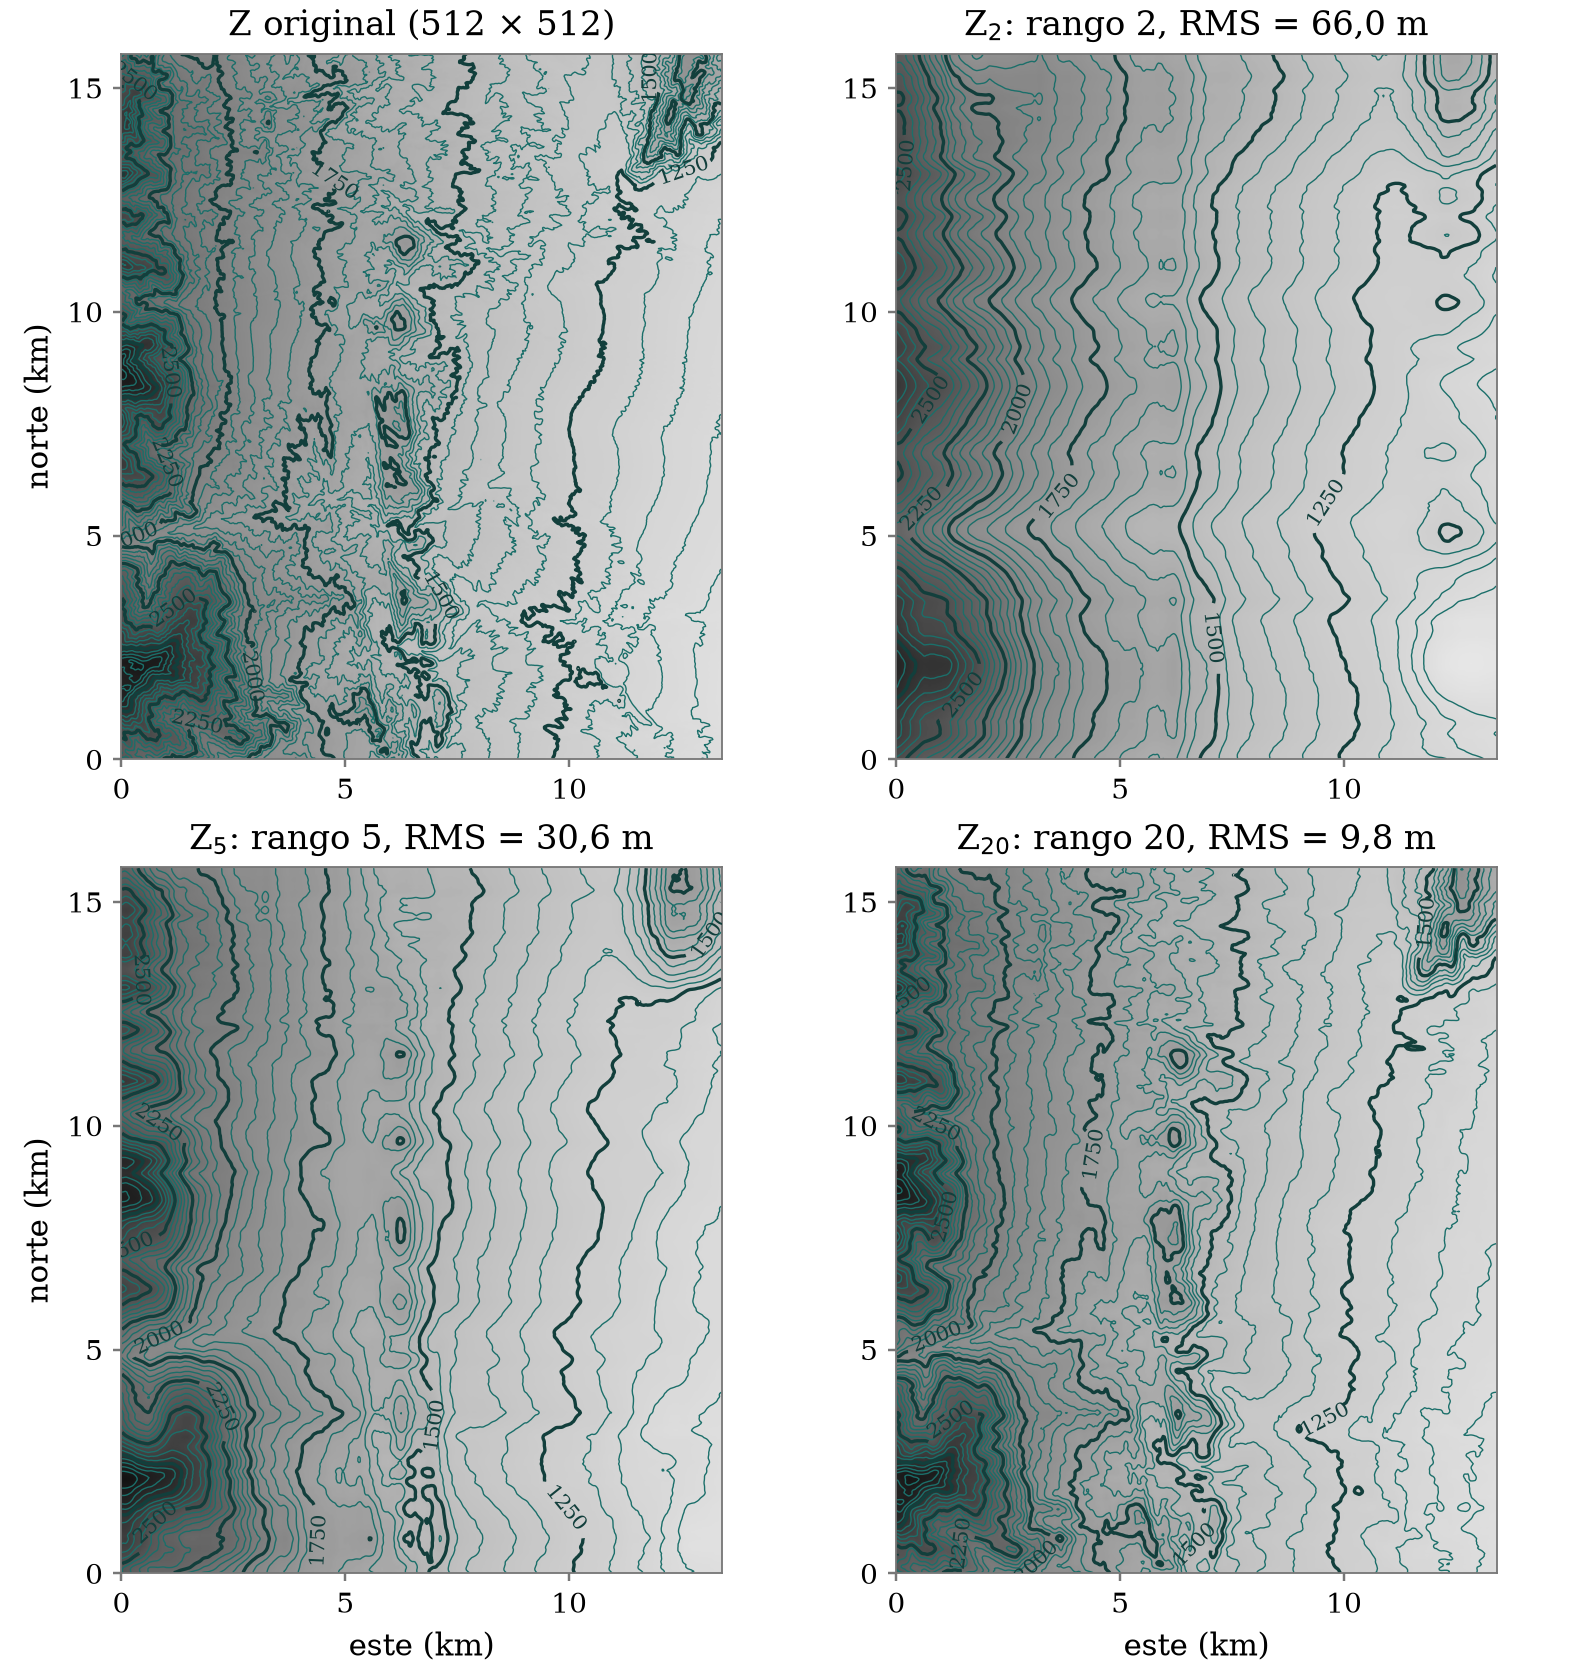
\includegraphics[width=\textwidth]{figuras/svd/dem_curvas_nivel.png}
\caption{Curvas de nivel del recorte de la Precordillera de Mendoza (Copernicus DEM GLO-30,
\(512\times512\) celdas de \(1''\)), equidistancia \(50\) m, maestras cada \(250\) m, trazadas
sobre el DEM original y sobre sus aproximaciones de rango \(2\), \(5\) y \(20\). El fondo gris
es la altura (más oscuro, más alto). Generada con
\texttt{apunte/figuras/svd/gen\_dem\_curvas\_nivel.py}.}
\label{fig:svd-dem-curvas}
\end{figure}

\paragraph{Lo que se ve.} Con \(k=2\) quedan las formas grandes: el cordón alto del oeste, el
descenso hacia el este y un par de lomas, todo con curvas de trazo largo y casi paralelas a
los meridianos. Es lo que cabe esperar de una suma de dos tejidos: cada uno tiene perfiles
norte--sur de una sola forma, de modo que las curvas tienden a alinearse con las columnas o con
las filas de la grilla. Ese sesgo es propio del método, no del terreno: un cordón oblicuo a la
grilla necesita muchos términos separables para quedar bien descripto. Con \(k=5\) aparecen
el cerro del ángulo noreste y los cerros del centro, todavía como manchas suaves. Con
\(k=20\) vuelve casi todo el dibujo: los cerros chicos alineados de norte a sur en el centro,
las entradas de las curvas en los cauces del oeste, los bordes quebrados de las maestras de
\(1500\) y \(1250\) m. Medido por el largo total de las curvas
de \(50\) m sobre el terreno, el DEM original tiene \(1174\) km de curvas repartidos en
\(307\) tramos; \(Z_{20}\) tiene \(923\) km en \(172\) tramos; \(Z_5\), \(716\) km en
\(119\); \(Z_2\), \(609\) km en \(83\). Cada término agregado agrega rugosidad, y una parte
de esa rugosidad es relieve y otra parte es ruido del propio DEM (es un modelo de superficie,
con vegetación y artefactos de medición, no de terreno desnudo).

\paragraph{Cuándo el filtro sirve y cuándo falsea.} Truncar la SVD es un filtro con una
ventaja clara: el error está controlado por números que conocemos antes de dibujar, los
\(\sigma_i\) descartados. Sirve cuando la escala del plano no puede mostrar el detalle: en
cartografía a escala chica, con equidistancia grande, las curvas del DEM original salen
temblorosas y llenas de tramos cortos que el dibujante igual eliminaría a mano, y \(Z_k\) los
elimina con un criterio uniforme en toda la hoja. Falsea cuando lo que se busca es justamente
el detalle local: el talud de un camino, una cárcava, el borde de una terraza, el pie de un
cerro que define un límite. Un error RMS bajo es un promedio sobre \(262\,144\) celdas y no
garantiza nada en una celda en particular: con \(k=20\) el RMS es \(9{,}8\) m pero el error
llega a \(75\) m en la peor celda, aunque sólo en el \(0{,}04\)\,\% de las celdas supera los
\(50\) m. Para un relevamiento de detalle, la matriz que manda es \(Z\), y conviene mirar
\(Z-Z_k\) como mapa para saber qué se está tirando.

\paragraph{Un criterio numérico para elegir \(k\).} Una curva de nivel está bien ubicada si
el error en altura es chico frente a la equidistancia: si el error vale la mitad de \(e\), la
curva puede confundirse con su vecina. Una regla práctica razonable es pedir
\[
  \mathrm{RMS}_k\le\frac{e}{5},
\]
y como \(\mathrm{RMS}_k\) se calcula sólo con los \(\sigma_i\), el menor \(k\) que la cumple
se busca recorriendo la lista de valores singulares. En el recorte de la Precordillera:

{\small
\begin{center}
\begin{tabular}{r r r r r}
\toprule
equidistancia \(e\) & tolerancia \(e/5\) & menor \(k\) & \(\mathrm{RMS}_k\) & error máximo\\
\midrule
\(100\) m & \(20\) m & \(9\) & \(18{,}7\) m & \(129\) m\\
\(50\) m & \(10\) m & \(20\) & \(9{,}8\) m & \(75\) m\\
\(25\) m & \(5\) m & \(44\) & \(4{,}95\) m & \(33\) m\\
\bottomrule
\end{tabular}
\end{center}
}

Para la equidistancia de la figura, \(50\) m, el criterio elige \(k=20\): veinte tejidos de
\(512\), y \(Z_{20}\) se guarda con \(20\cdot(512+512+1)=20\,500\) números en lugar de
\(262\,144\), menos del \(8\)\,\%. El error en altura se traduce en un corrimiento horizontal
de la curva que depende de la pendiente: donde el terreno sube \(\tan\theta\) metros por
metro, un error vertical \(\delta\) corre la curva unos \(\delta/\tan\theta\) metros. La
pendiente mediana del recorte es \(0{,}188\) (unos \(10{,}6^\circ\)), así que los \(9{,}8\) m
de \(Z_{20}\) mueven las curvas del orden de \(52\) m, dos celdas, en un terreno típico, y
bastante más en los llanos del este, donde la pendiente es menor. Es el mismo número visto de
otro modo: en escala \(1\!:\!50\,000\), \(52\) m son un milímetro del plano, el límite de lo
que se dibuja; en escala \(1\!:\!5000\) son un centímetro, y ahí \(k=20\) ya no alcanza.

\subsubsection{Conexiones con el resto del programa}\label{sec:svd-dem-conexiones}

\paragraph{El plano de ajuste y la pseudoinversa.} El primer modelo de un terreno que se le
ocurre a un agrimensor no es \(Z_1\) sino un plano, \(z=a\,x+b\,y+c\), con \(x\) hacia el este
y \(y\) hacia el norte en metros. Ajustarlo es un sistema sobredeterminado de \(262\,144\)
ecuaciones con tres incógnitas, una por celda, \(a\,x_j+b\,y_i+c\approx z_{ij}\), que se
resuelve con la pseudoinversa de la sección~\ref{sec:pseudoinversa}: \((a,b,c)=A^{+}z\), con
\(A\) de \(262\,144\times3\) y columnas \(x\), \(y\) y unos. En el recorte da un plano que baja
\(97\) m por kilómetro hacia el este y sube \(4{,}4\) m por kilómetro hacia el norte
(pendiente de \(5{,}5^\circ\)), con un RMS de \(153{,}7\) m.

La comparación con la SVD es instructiva. El plano, escrito como matriz, es
\((b\,y_i+c)\cdot1+a\cdot x_j\): la suma de una matriz que sólo depende de la fila y otra que
sólo depende de la columna, de rango dos. Por lo tanto su error no puede ser menor que el de la
mejor aproximación de rango dos, y efectivamente \(153{,}7\ \text{m}>66{,}0\ \text{m}\). Lo
llamativo es que también pierde contra \(Z_1\), de rango uno, que da \(102{,}9\) m. La razón
es que el plano obliga a los perfiles a ser rectas, mientras que la SVD elige los perfiles que
mejor describen el terreno, y el perfil oeste--este real, que cae más de \(1400\) m en
\(13\) km de manera nada uniforme, no es una recta. Los dos ajustes son mínimos cuadrados con
el mismo dibujo de la proyección ortogonal (caja ``El dibujo único detrás de \(Ax\approx b\)''
de la sección~\ref{sec:cuatro-problemas}); lo que cambia es el subespacio sobre el que
proyectamos: planos en un caso, matrices de rango \(k\) en el otro.

\paragraph{La grilla geográfica no es cuadrada.} Todo lo anterior trató a \(Z\) como una
tabla con celdas iguales, y la SVD lo hace sin preguntar: suma cuadrados de alturas celda por
celda. Pero las celdas de un segundo de arco no son cuadradas (\(30{,}80\) por \(26{,}19\) m
en este recorte) ni todas iguales: el ancho este--oeste es \(N\cos\varphi\) por un segundo
en radianes, con \(N\) la gran normal del elipsoide, y pasa de \(26{,}17\) m en el borde sur a
\(26{,}21\) m en el borde norte. En \(15\) km la variación es despreciable; en un DEM que cubre
varios grados de latitud no lo es, y una celda cerca del polo es una astilla. La grilla
\((\lambda,\varphi)\) es una parametrización del elipsoide con primera forma fundamental
\(ds^2=N^2\cos^2\varphi\,d\lambda^2+M^2\,d\varphi^2\) (secciones~\ref{sec:metrica}
y~\ref{sec:elipsoide}). Para las curvas de nivel eso tiene dos consecuencias. El trazado
mismo no cambia, porque una curva de nivel es el núcleo de una forma y no necesita métrica.
Cambian todas las cuentas que miden: el largo de las curvas, las pendientes, la dirección de
máxima pendiente y el corrimiento horizontal de una curva por un error vertical, que en este
recorte hicimos convirtiendo celdas a metros con los dos factores de la métrica. Y si
quisiéramos que la propia SVD pesara cada celda por el área que representa, habría que
descomponer \(D_1^{1/2}\,Z\,D_2^{1/2}\), con \(D_1\) y \(D_2\) diagonales con los pesos de
filas y columnas: otra vez, la base privilegiada la elige la regla de medir.

\begin{resultado}[Lo que sabemos hacer con un modelo digital de elevación]
Leerlo como matriz \(Z\) y como muestra de una función \(z=f(x,y)\) en una grilla geográfica.
Descomponerlo en tejidos separables \(\sigma_iu_iv_i^T\) y saber, sólo con los \(\sigma_i\)
descartados, el error RMS en metros de la aproximación \(Z_k\). Trazar sus curvas de nivel
celda por celda por interpolación lineal, sabiendo que cada tramo aproxima la recta de nivel
cero del plano tangente. Y elegir \(k\) para que el error quede por debajo de una fracción de
la equidistancia (en la Precordillera, \(k=20\) para \(50\) m), sabiendo que el filtro sirve
para la forma grande y no para el detalle de un relevamiento.
\end{resultado}
